%% -*- coding: utf-8 -*-
\documentclass[12pt,pagesize,paper=192mm:108mm]{scrbook} 
%1920x1080 1280x720
\areaset[current]{192mm}{108mm}
\usepackage{calc}
\usepackage[T2A]{fontenc}
\usepackage[utf8]{inputenc}
\usepackage[english,russian]{babel}
\usepackage{microtype}
\usepackage{misccorr}
\usepackage{cmap}
%\usepackage[unicode=true]{hyperref}
\usepackage{graphicx}
\usepackage{amssymb}
\usepackage{amsmath}
%\usepackage{srcltx}
\usepackage{textcomp}
\usepackage{xspace}
%научные символы и смайлики \smiley \frownie
\usepackage{wasysym}
\usepackage{ccicons}
\begin{document}
\begin{titlepage}
  \vspace*{-0.5em}
  \begin{center}    
    \hspace*{3em}
    \begin{minipage}[t]{3em}
      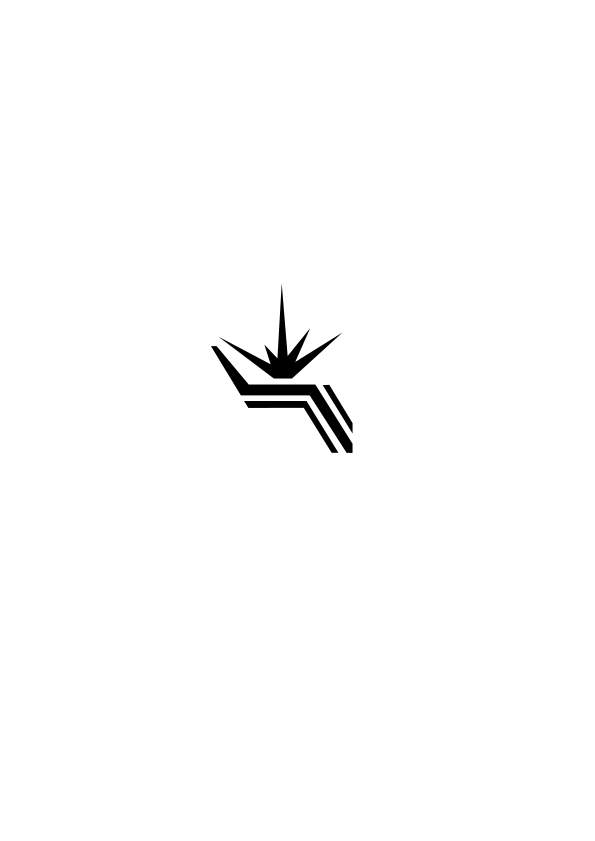
\includegraphics[width=\textwidth]{../BINP-logo}
    \end{minipage}\hfill
    \begin{minipage}{0.23\linewidth}
    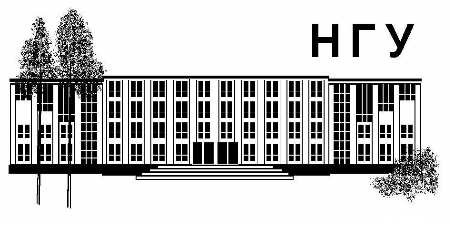
\includegraphics[width=\textwidth]{../NSU-logo}
    \end{minipage}
    \hfill
    \hspace*{6em}

    Кафедра теоретической физики физического факультета НГУ
    \medskip

    \Large
    Профессор Черняк В.\,Л.
    \bigskip

    \huge
    \textbf{Теория электрослабых взаимодействий}
    \bigskip

    \Large
    Лекция № 17
    \vfill

    % \normalsize
    % \begin{minipage}{0.65\linewidth}
    % \end{minipage}
    \vfill

\normalsize    Новосибирск 2013
  \smallskip

  \ccbysa
  \end{center}
\end{titlepage}
\newpage

\vspace*{-1em}
\begin{center}
 \vfill
  \begin{minipage}{0.66\linewidth}
    $CP$"=нарушение. Параметризация $CP$"=нарушения в матрице CKM:
    параметры $\beta$ и $\gamma$.  Типы $CP$"=нарушения: прямое
    $CP$"=нарушение и $CP$"=нарушение за счёт смешивания нейтральных
    мезонов.  $B^0-\bar{B}^0$ осцилляции во втором порядке теории
    возмущений: $\Delta F = 2$ переходы (изменение флейвора на
    2). Прямое $CP$"=нарушение. Распад $B^-\to K^-\pi^0$ и $B^+\to
    K^+\pi^0$.  Трудности описания сильных ($CP$"=чётных) фаз
    амплитуды. Древесные и пингвинные вклады. Разность парциальных
    ширин распадов $B^-\to K^-\pi^0$ и $B^+\to K^+\pi^0$.
    $CP$"=нарушение за счёт смешивания нейтральных мезонов. Массовая
    матрица для $B^0-\bar{B}^0$ смешивания.  Матричный элемент
    $M_{12}$ в приближении факторизации. Разности масс для собственных
    состояний массовой матрицы.  Соотношение унитарности, мнимая часть
    массовой матрицы, ширины распадов $B$"=мезонов. $B$"=фабрики и
    определение угла $\beta$. Золотая мода.  Распад $B^0\to J/\psi
    K_S$ ($\bar{B}^0\to J/\psi K_S$).  Малость пингвинных вкладов в
    золотой моде. Тагирующая мода в распадах $B^0$ и $\bar{B}^0$.
  \end{minipage}
  \vfill
  % Новосибирск 2013

  % \normalsize \ccbysa
\end{center}
\end{document}
